\documentclass{ufscThesis/ufscThesis} % Definicao do documentclass ufscThesis	

%----------------------------------------------------------------------
% Pacotes usados especificamente neste documento
\usepackage{graphicx} % Possibilita o uso de figuras e gráficos
\usepackage{color}    % Possibilita o uso de cores no documento
\usepackage{listings}


\usepackage{amsmath}
\usepackage{multirow}
\usepackage{url}
%\usepackage{hyperref}
%----------------------------------------------------------------------
% Comandos criados pelo usuário
\newcommand{\afazer}[1]{{\color{red}{#1}}} % Para destacar uma parte a ser trabalhada

%----------------------------------------------------------------------
% Identificadores do trabalho
% Usados para preencher os elementos pré-textuais
\instituicao[a]{Universidade Federal de Santa Catarina} % Opcional
\departamento[a]{INE}
\curso[a]{Universidade Federal de Santa Catarina}
\documento[a]{Tese} % [o] para dissertação [a] para tese
\titulo{Portando o EPOS para a Zedboard}
%\subtitulo{Subtítulo (se houver)} % Opcional
\autor{Bruno Farias de Loreto}
\grau{Bacharel em Ciências da Computação}
\local{Florianópolis} % Opcional (Florianópolis é o padrão)
\data{22}{Fevereiro}{2014}

\orientador[Orientador\\Universidade Federal de Santa Catarina]{Prof. Dr. Antônio Augusto Fröhlich}
\coorientador[Coorientador\\Universidade Federal de Santa Catarina]{Prof. M.Sc. Giovani Gracioli}
\coordenador[Coordenador\\Universidade Federal de Santa Catarina]{Prof. Dr. Vitório Bruno Mazzola}

\numerodemembrosnabanca{4} % Isso decide se haverá uma folha adicional
\orientadornabanca{nao} % Se faz parte da banca definir como sim
\coorientadornabanca{sim} % Se faz parte da banca definir como sim
\bancaMembroA{Arliones Stevert Hoeller Junior\\Universidade Federal de Santa Catarina}
\bancaMembroB{Hugo Marcondes\\Universidade Federal de Santa Catarina}
%\bancaMembroC{... \\...}     % Nome do membro da Banca
%\bancaMembroD{... \\...}       % Nome do membro da Banca
%\bancaMembroE{Quinto membro\\Universidade ...}       % Nome do membro da Banca

%\dedicatoria{Este trabalho é dedicado a ...}

\agradecimento{Agradeço àquele que morreu e ressucitou por nós, Goku!}

\epigrafe{So long, and thanks for all the fish!\\\emph{- Douglas Adams.}}
%{(Autor da epígrafe, ano)}

\textoResumo {
	No mundo dos sistemas operacionais embarcados, há uma grande variedade de diferentes arquiteturas, e, consequentemente, um sistema operacional embarcado necessita dar suporte a um bom número de arquiteturas para ser usável em diversos cenários. 
	O sistema operacional EPOS possui uma arquitetura que tenta ser o mais independente de plataforma possível, entretanto o interfaceamento entre o software e hardware inevitavelmente necessita ser reescrito.
	Este trabalho visa descrever e documentar como o sistema operacional EPOS foi portado para a Zedboard, uma plataforma ARM \emph{multicore}.
}
\palavrasChave {Systemas Operacionais. Portabilidade. EPOS.}
 
\textAbstract {
	
}
\keywords {Operating Systems. Porting. EPOS.}

%----------------------------------------------------------------------
%Para gerar a lista de símbolos e abreviaturas use os comandos
%
%\simbolo{$\int$}{Integral}
%\simbolo{$\prod$}{Produtório}
%
%\begin{lstlisting}
%\simbolo{símbolo}{descrição}
%\end{lstlisting}
%
%\begin{lstlisting}
%\abreviatura{abreviatura}{descrição}
%\end{lstlisting}
%Segundo \citeonline{alves_2001} ...
%--------------------------------------------------------

\begin{document}

%\capa  
\folhaderosto%[comficha] % Se nao quiser imprimir a ficha, é só não usar o parâmetro
\folhaaprovacao
\paginadedicatoria
\paginaagradecimento
\paginaepigrafe
\paginaresumo
\paginaabstract
%\pretextuais % Substitui todos os elementos pre-textuais acima
\listadefiguras % as listas dependem da necessidade do usuário
\listadetabelas 
\listadeabreviaturas
%\listadesimbolos
\sumario

\abreviatura{SoC}{\emph{System-on-Chip}.}
\abreviatura{TCM}{\emph{Tightly Coupled Memory}}
\abreviatura{MMU}{\emph{Memory Management Unit}}
\abreviatura{SP}{\emph{Stack Pointer}}
\abreviatura{PC}{\emph{Program Counter}}
\abreviatura{LR}{\emph{Link Register}}
\abreviatura{CPSR}{\emph{Current Program Status Register}. O registrador que armazena o atual status do processador operante.}
\abreviatura{SPSR}{\emph{Saved Program Status Register}. (Registrador que armazena o valor de CPSR no momento imediatamente anterior ao acontecimento de uma exceção, deste modo o antigo valor de CPSR pode ser restaurado quando a exceção for tratada.}
\abreviatura{CP15}{\emph{System Control Coprocessor}}
\abreviatura{IRQ}{Interrupção normal.}
\abreviatura{FIQ}{\emph{Fast Interrupt}.}
%\abreviatura{SCR}{\emph{ }}
\abreviatura{APSR}{\emph{Application Program Status Register}. Armazena uma cópia do estado das \emph{flags} da unidade lógico-aritimética. Conhecido também como \emph{flag} do código condicional, usados para determinar se uma instrução condicional deve ser executada ou não.}
\abreviatura{GIC}{\emph{Generic Interrupt Controler}}
\abreviatura{rx}{Quando a abreviação rx aparecer, ela estará se referindo genericamente à qualquer um dos 13 primeiros registradores de propósito geral do ARM9 [r0-r12].}
\abreviatura{PPI}{\emph{Private Peripheral Interrupt.}}
\abreviatura{SGI}{\emph{Software Generated Interrupt.}}
\abreviatura{SPI}{\emph{Shared Peripheral Interrupt.}}
\abreviatura{PS}{\emph{Processing system.}}
\abreviatura{PL}{\emph{Programmable Logic.}}
\abreviatura{SMC}{\emph{Static Memory Controller}}
\abreviatura{TSC}{\emph{Time Stamp Counter.}}
\abreviatura{FPGA}{\emph{Field-Programmable Gate Array}. Hardware reconfigurável, o qual têm as suas funcionalidades definidas exclusivamente pelos usuários.}
\abreviatura{PLL}{\emph{Phase-Locked Loop}. É um sistema de controle que gera uma saída cuja fase é relacionada à fase do sinal de entrada. Pode ser usada para estabilizar um sinal e também multiplica-lo.}
\abreviatura{SCU}{\emph{Snoop Control Unit}.}
%--------------------------------------------------------
% Elementos textuais

\chapter{Introdução}

O presente trabalho visa descrever como foi feito o porte\footnote{Porte é um estrangeirismo da palavra \emph{port}, que, no âmbito da computação, significa o ato de fazer um mesmo programa/sistema/SO funcionar em diferentes ambientes. Por exemplo, fazer um software que antes só funcionava no Linux passar a funcionar em um outro SO (sistema operacional) pode ser considerado um porte. Uma palavra alternativa que poderia ser usada é ``suporte'', entretanto acredito que esta palavra não expresse apropriadamente o que foi feito, já que essa palavra normalmente é associada com um serviço pago de assistência técnica, e o próprio fraseamento do que foi feito se tornaria de mais difícil compreensão e prolixo com esta palavra.} do sistema operacional EPOS para a plataforma Zedboard, bem como comentar sobre as decisões tomadas e problemas enfrentados.

\section{Motivação}
EPOS é um sistema operacional que visa reduzir o custo de produção das aplicações embarcadas provendo um ambiente onde a aplicação do desenvolvedor possa rodar sem que ele tenha que lidar com configurações de baixo nível. Sendo assim é importante que o EPOS seja portado para um grande número de plataformas, do contrário sua utilidade prática seria prejudicada.

Zedboard é uma plataforma que usa o SoC Xilinx 7000, que por sua vez possui o processador \emph{dual core} ARM Cortex A9. Existe uma dupla motivação para se fazer o porte para esta plataforma: Primeiro que o EPOS ainda não foi portado para um processador RISC \emph{multicore}, e acredita-se que este porte poderá possibilitar linhas de pesquisa com o EPOS que antes só poderiam ser feitos num CISC, algo que não é o ideal considerando-se o nicho de aplicação do EPOS. O segundo fator está relacionado com o próprio Zedboard. Dentro do LISHA (Laboratório de Integração Software-Hardware) há uma linha de pesquisa sobre Smart Homes (ou Smart Buildings) em cujo contexto se pretende usar um Zedboard.

\section{Objetivos Gerais}

O objetivo deste trabalho é portar o sistema operacional EPOS e documentar este processo no presente documento. O porte consiste em adaptar os componentes que, dentro da arquitetura do EPOS, são chamados de mediadores de hardware. Cada mediador precisa ser refeito para cada plataforma.
Este trabalho terá certo direcionamento para as pessoas que no futuro precisem fazer um novo porte do EPOS, de modo que elas não precisem passar pelos mesmos problemas e possam, portanto, fazer isto mais eficientemente.

\section{Objetivos Específicos}
Dos objetivos específicos, pode-se organizá-los da seguinte forma:

\begin{enumerate}
    \item Estudo da arquitetura do EPOS, da arquitetura do ARM Cortex A9 e do Zedboard.
    \item Portes
    \begin{enumerate}
        \item Timers
        \item Controlador de Interrupção
        \item MMU
        \item CPU
        \item Inicialização elf e Multicore
    \end{enumerate}
    \item Validações
    \begin{enumerate}
        \item Escalonadores em single e multicore
        \item Threads
        \item Thread Periódica
        \item Alarmes
        \item Cronômetro
        \item Sincronização
    \end{enumerate}
    \item Documentação
\end{enumerate}

\chapter{Conceitos Básicos}

%source: http://epos.lisha.ufsc.br/EPOS+User+Guide
\section{EPOS}

EPOS (Embedded Parallel Operating System) é um sistema operacional orientado a aplicação, cujo design chama-se ADESD (\emph{Application-Driven Embedded System Design Method}), proposto por Fröhlich \cite{guto_thesis}. A ideia central do EPOS é prover um sistema operacional mínimo, de modo a minimizar o \emph{overhead} da existência de um sistema operacional, deixando o processador livre para executar a aplicação do desenvolvedor \cite{epos_user_guide}.

Como o objetivo é criar um ambiente em que o desenvolvedor possa rapidamente produzir suas aplicações, EPOS provê vários utilitários comumente usados em aplicações, como filas, listas, tabelas de hashs, vetores, semáforos, OStream (para imprimir na tela), números aleatórios, cálculo de CRC e etc. Além destes utilitários, EPOS também provê uma série de componentes como threads, alarmes, cronometros, heaps e meios para acessar a rede (internet).

\section{Arquitetura do EPOS}

\textbf{Mediadores de Hardware:} Dentro da arquitetura do EPOS há o conceito de mediadores de hardware, que são os componentes (ou classes) dependentes de plataforma. Idealmente, as únicas classes que precisam ser modificadas e/ou reimplementadas são os mediadores. Há mediadores específicos da placa, como por exemplo Pandaboard, Zedboard e etc; abstraídos sob o nome de \emph{machine} e mediadores específicos de um processador, abstraídos sob o nome de \emph{architecture}. No código do EPOS, estes mediadores encontram-se nas pastas \emph{mach} e \emph{arch}.
% Fonte: Hardware Mediators: A Portability Artifact for Component-based Systems
% HAL vs Virtualização vs Mediadores

Mediadores de hardware são uma alternativa ao tradicional uso de VMs\footnote{Virtual Machines.} e de HAL\footnote{Hardware Abstraction Layer}, proposta por Fröhlich em seu trabalho \emph{Application-Oriented System Design} \cite{guto_thesis}. O problema do uso de VMs é o seu \emph{overhead} causado devido à tradução das operações da VM em código nativo. Já o uso de um HAL incorre no problema da manutenibilidade e dificuldade de adapção à novas arquiteturas muito distintas entre si \cite{hw_mediators}. O HAL não conseguiu passar pela prova do tempo, e já está sendo considerado obsoleto por distribuições GNU/Linux populares, como o 
Ubuntu\footnote{\url{http://www.linux-magazine.com/Online/News/Ubuntu-10.04-Alpha-2-Removes-HAL}}, sendo chamado de ``uma grande não-manutenível bagunça monolítica''\footnote{\url{https://wiki.ubuntu.com/Halsectomy}}.



\textbf{Traits:} Traits é uma classe onde é possível configurar certos componentes do EPOS em tempo de compilação. Lá é possível, por exemplo, definir o tamanho da stack e heap do sistema, a sua frequência de clock bem como ativar ou desativar certas funções do sistema. Esta classe normalmente precisa ser alterada em um porte, mesmo ela não sendo um mediador de hardware.

\textbf{Interface Infladas: } Um conceito importante da arquitetura do EPOS é a Interface Inflada. %http://www.inf.ufsc.br/~guto/publications/aoos.pdf
Em sistemas orientados a aplicação, famílias de abstrações são frequentemente tratadas como entidades únicas, algo que pode ser vantajoso para o programador da aplicação, já que este não precisaria se preocupar com qual membro em específico desta família ele precisaria usar\cite{guto_thesis}.

Interface inflada basicamente é uma interface que declara os métodos de todas as classes que derivam dela, exportanto assim todos os métodos daquela família de abstrações. Deste modo, o desenvolvedor de aplicativo poderia escrever a aplicação inteira em termos da interface inflada, relegando a tarefa de configuração do sistema a um utilitário automatizado. Tal utilitário poderia, através de uma análise sintática do código fonte, escolher quais os membros mais leves da família exportada serão associados no momento da compilação \cite[p.~56]{guto_thesis}.

%write about specifics from timers
\begin{figure}[ht!]
    \centering
    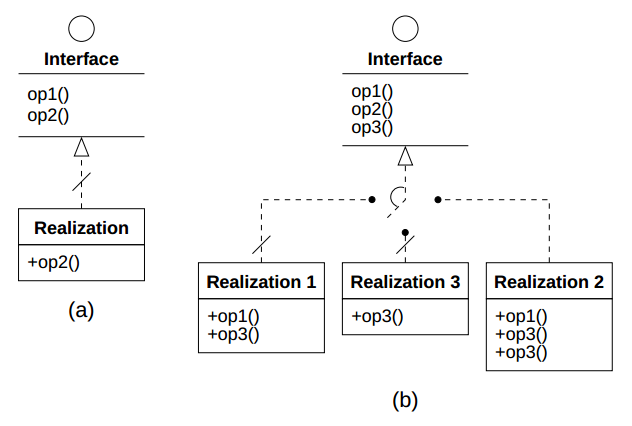
\includegraphics[width=7.5cm]{figuras/inflated_interface}
    \caption{Exemplos de uso de interfaces infladas \cite{guto_thesis}.}
\end{figure}


\section{Hardware-alvo}
%source: http://www.zedboard.org/product/zedboard
% http://www.zedboard.org/sites/default/files/documentations/ZedBoard_HW_UG_v2_2.pdf
Zedboard é uma plataforma de desenvolvimento que suporta uma grande variedade de aplicações, visto que ela possui uma boa gama de interfaces e funções para habilitar isto. É dedicada à prototipação e \emph{proof-of-concept}. Em seu interior ela possui um Xilinx Zynq 7000 (Z-7020), que é a arquitetura alvo deste porte.

O ZYNQ-7000 SOC XC7Z020-CLG484-1 conta com o processador Dual ARM Cortex-A9 MPCore. O Zynq possui 4 graduações de velocidade de \emph{clock}, a comercial (graduação -1), industrial (graduação -1 a -2), estendida (-2 a -3) e expandida (-1), sendo a graduação -1 a menor velocidade, e a -3 a maior \cite{product_table}.

De acordo com a especificação da Zedboard \cite{zedboard}, o \emph{clock} máximo do processador é de 667MHZ, portanto, tendo como referência a tabela de dados do Zynq-7000 \cite[p.~13]{data_sheet}, chegamos à conclusão que a graduação de velocidade do Zynq usado na Zedboard é de -1 (comercial), esta informação se tornará útil mais à frente.

Há disponível 512MB de RAM DDR3, e um SD card de 4GB. A Zedboard suporta conexão com JTAG, saída serial (USB UART) e conexão com a internet \cite{xilinx}.

A família Zynq 7000 disponibiliza para o desenvolvedor FPGAs, tornando esta plataforma mais configurável e flexível \cite[p.~26]{ug585}. A PS dessa família é a mesma para cada dispositivo onde ela se encontra, entretanto a PL e recursos de entrada e saída variam entre diferentes dispositivos. 


\begin{figure}[ht!]
    \centering
    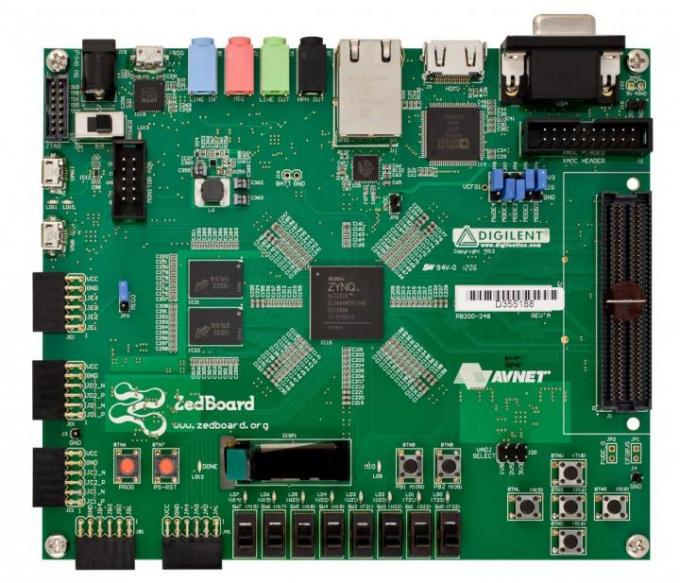
\includegraphics[width=8cm]{figuras/zedboard}
    \caption{Zedboard visto de cima.}
\end{figure}

\subsection{Arquitetura do Zynq 7000}
Como já citado, o Zynq 7000 possui um processador \emph{dual core}Cortex A9, cada core possui sua própria MMU e memória cache L1 (instruções e dados) privada.

%layout de memoria
\subsection{OCM} O \emph{On-chip Memory} é uma pequena memória de 256KB de RAM que fica próxima ao processador, e portanto tem um acesso mais rápido. O OCM pode ser mapeado nos primeiros 256KB do espaço de endereçamento, ou nos últimos 256KB do espaço de endereçamento \cite{ug585}, como mostrado na tabela \ref{tab.memlayout}.


\subsection{Modos de Operação}
\label{sec:operating_modes}
A arquitetura ARMv7 conta com 9 modos de operação (7 por padrão, mais 2 com extensões habilidadas), sendo que o único modo não privilegiado é o modo de usuário, os demais modos padrão possuem o mesmo privilégio dentro do sistema. A principal diferença entre um modo e outro é que cada modo conta com um certo subconjunto privado de registradores, visiveis somente no modo em vigência, detalhes sobre estes registradores seguem na seção seguinte. A tabela abaixo ilustra quais são os modos de operação disponíveis \cite[p.~1139]{armarm}.
O campo ``Codificação'' é usado no registrador CPSR para se verificar ou modificar o modo de operação.

\begin{table}[ht]
\centering
\begin{tabular}{ccc}
\hline\hline                        %inserts double horizontal lines
Modo do processador  & Codificação & Implementado?\\ [0.5ex] % inserts table 
%heading
\hline                  % inserts single horizontal line
User & 10000 & Sempre \\
FIQ & 10001 & Sempre \\
IRQ & 10010 & Sempre \\
Supervisor & 10011 & Sempre\\
Monitor & 10110 & Com extenções de segurança.\\
Abort & 10111 & Sempre\\
Hyp & 11010 & Com extenções de virtualização.\\
Undefined & 11011 & Sempre\\
System & 11111 & Sempre\\[1ex]
\hline %inserts single line
\end{tabular}
\caption{Modos do processador.}
\label{tab.processormode} % is used to refer this table in the text
\end{table}

\textbf{Modo Usuário:} Modo não-privilegiado de execução. Neste modo somente é possível de se fazer acesso não privilegiado aos recursos do hardware (não prodendo acessar as áreas protegidas). Não é possível de se mudar para outro modo de operação quando neste, a não ser por eventos externos como interrupções.

\textbf{Modo Sistema:} Modo privilegiado de execução. Este modo usa os mesmos registradores que o modo usuário e nenhuma exceção leva a este modo. Somente é possível de se entrar nesse modo alterando os bits do registrador de status do sistema (CPSR); é necessário já estar em algum modo privilegiado para tal operação.

\textbf{Modo Supervisor:} É o modo padrão para no qual processador entra quando exceção do tipo \emph{Supervisor Call} é recebida.
Para gerar um \emph{Supervisor Call}, usa-se a instrução \verb+svc+. O processador entra neste modo ao se resetar.

\textbf{Modo Abort:} Modo que o processador entra quando recebe uma interrupção do tipo \emph{prefetch abort} ou \emph{data abort}.

\textbf{Modo Indefinido:} Modo que o processador entra quando se tenta executar uma instrução não definida.

\textbf{Modo FIQ:} Modo que o processador entra quando recebe uma interrupção FIQ.

\textbf{Modo IRQ:} Modo que o processador entra quando recebe uma interrupção IRQ.

\textbf{Modo Hipervisor:} Este modo possui ainda mais privilégios que os demais modos, mas somente existe quando as extenções de virtualização estão ativas (fora do escopo deste trabalho).

\textbf{Modo Monitor:} Modo que o processador entra quando recebe uma interrupção \emph{Secure Monitor Call}, \verb+SMC+. Este modo está fora do escopo do trabalho.


\begin{figure}[ht!]
	\centerline{
    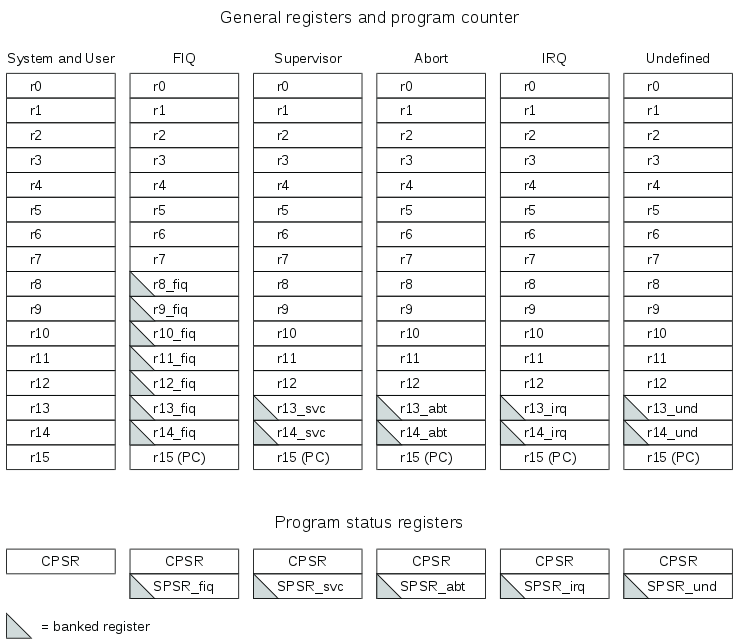
\includegraphics[width=12cm]{figuras/banked_registers}
	}
    \caption{Banked registers.}
\end{figure}



\subsection{GIC}
O GIC (\emph{Generic Interrupt Controller}) é um componente que centraliza e administra todas as interrupções do sistema, ativando, desativando, mascarando e priorizando as fontes de interrupção.


\subsection{Tipos de Interrupção} %ug585 p. 192
\label{sec:interrupt}
\textbf{Interrupção Gerada por Software: }
Cada CPU pode se interromper, interromper outra CPU, ou ambas CPUs usando SGIs (\emph{Software Generated Interrupts}). Existem 16 interrupções geradas por software, que podem ser geradas escrevendo o número da interrupção ([0-15]), junto com o número da CPU alvo no registrador ICDSGIR. Esta escrita ocorre dentro do barramento privado da própria CPU. Cada CPU possui seu próprio conjunto privado de registradores de SGIs para gerarem uma (ou mais) das 16 SGIs possíveis. É possível limpar uma interrupção lendo o registrador ICCIAR (\emph{Interrupt Acknowledge}) ou escrevendo 1 nos bits correspondentes do registrador ICDICPR (\emph{Interrupt Clear-Pending}).
\\\\
\textbf{Interrupções de Periféricos Privados da CPU: }
Cada CPU está conectada a um conjunto privado de 5 interrupções de periféricos, são eles: Relógio Global (\emph{Global Timer}), nFIQ (\emph{Fast Interrupt}), Relógio privado da CPU, \emph{Watchdog} privado da CPU e nIRQ (interrupção vinda da lógica programável).
\\\\
\textbf{Interrupções de Periféricos Compartilhados: }
Existem cerca de 60 interrupções de diversos modulos que podem ser roteadas para um ou ambos processadores, ou para a lógica programável. O GIC é responsável por administrar estas interrupções.

\begin{figure}[ht!]
	\centerline{
    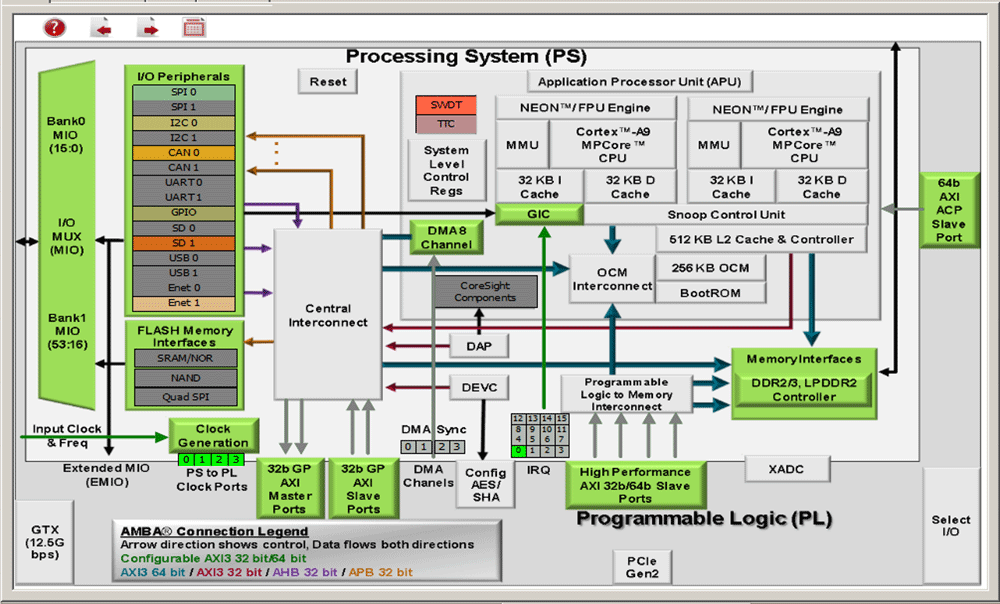
\includegraphics[width=13cm]{figuras/zynq-7000}
	}
    \caption{Diagrama de blocos dos \emph{clocks} disponíveis no Zynq. Note os \emph{clocks} da tabela \ref{tab:clocks} no canto superior direito da imagem.}
\end{figure}

Há também as interrupções\footnote{Na nomenclatura do manual, usa-se o termo exceção para os 6 diferentes tipos de interrupção, e de interrupção os diferentes tipos de interrupção IRQ ou FIQ (as categorias de interrupção descritas acima são do tipo IRQ). Durante este trabalho preferiu-se usar apenas o nome interrupção, pois assim não há ambiguidade com a palavra exceção no contexto de linguagens de programação.} geradas por alguma exceção, i.e. algum evento inesperado no fluxo de execução. Além das interrupções IRQ (contempladas acima) existem mais 5 tipos interrupções que devem ser contempladas. São elas:

\textbf{FIQ \emph{Fast Interrupt}:} O modo FIQ possui um número maior de registradores banqueados que os demais modos (R8 até R13, além do SP, LR e SPSR), fazendo com que não seja necessário fazer troca de contexto. FIQs também tem mais alta prioridade que qualquer IRQ, pontanto este tipo de interrupção é apropriado para aplicações de tempo real de usuário único. Se multiplas aplicações tempo real usarem FIQ, pode haver conflitos de interesse que podem fazer um processo perder um \emph{deadline} \cite[p.~66]{armarm}.

%FIQ mode is designed for efficient use by a single owner, using R8_fiq – R13_fiq as global variables. 
%In addition, unlike IRQs, FIQs are not disabled by other exceptions (apart from reset), making them 
%the preferred type for real time interrupts, when other exceptions are being used routinely, such as 
%virtual memory or instruction emulation. IRQs may be disabled for unacceptably long periods of time 
%while these needs are being serviced.
%However, if more than one real-time interrupt source is required, there is a conflict of interest. The 
%new mechanism allows multiple FIQ sources and minimizes the period with FIQs disabled, greatly 
%reducing the interrupt latency penalty. The FIQ mode registers can be allocated to the highest priority 
%FIQ as a single owner
%ARM ARM p. 66.

\textbf{Instrução não definida \emph{Undefined Instruction}:} 
Há duas situações que geram esta interrupção: Quando se executa instruções de coprocessador que não são reconhecidas por este, ou quando se executa instruções que não possuem significado para o processador \cite[p.~36]{armarm}. Normalmente este tipo de interrupção acontecerá quando o processador estiver lendo e tentando executar lixo de memória.


\textbf{\emph{Prefetch Abort: }} Interrupção que leva ao modo Abort. Este tipo de interrupção é sinalizado pelo sistema de memória (MMU). Através da MMU, é possível de se marcar certas regiões de memória como não executáveis; isto é importante de se fazer em regiões de memória que possuem dados sensíveis, de modo que quando o processador tentar ler aquela área para executar num futuro próximo, a MMU envia um sinal invalidando aquilo que foi lido. Quando o processador tenta executar uma instrução que tenha sido anteriormente invalidada, uma interrupção do tipo \emph{prefetch} ocorre \cite[p.~58]{armarm}. Note que é possível do processador ler aquela região para executar em seguida, mas ainda não gerar esta interrupção; isto ocorre quando o fluxo é desviado antes da tentativa de executar aquela instrução (por um \emph{branch} por exemplo).

\textbf{\emph{Data Abort:}} Assim como a \emph{prefetch abort}, esta interrupção também leva ao modo Abort (e somente estas duas interrupções). Este tipo de interrupção pode acontecer quando uma instrução tenta acessar uma região de memória que o modo atual de execução não tenha permissão para acessar. Acesso a regiões de memória virtual não mapeadas pela MMU também geram esta interrupção.


%Source: http://infocenter.arm.com/help/index.jsp?topic=/com.arm.doc.dui0068b/BABFCEEG.html
\textbf{Interrupção de Software: } Existe uma instrução no assembly do ARMv9 que permite que seja feita uma interrupção de software (\verb+swi+). Esta instrução pode ser acompanhada de um número de 8 bits, significando que é possível se criar 256 interrupções de software diferentes. Esta interrupção leva ao modo supervisor.

\subsection{(\emph{Timers})}
Cada um dos \emph{cores} possui um \emph{timer} privado de 32 bits e ambos \emph{cores} compartilham um \emph{timer} global de 64 bits. Estes \emph{timers} trabalham numa frequ�ncia sempre igual � metade da frequ�ncia da CPU.
No n�vel de sistema (\emph{sistem-level (PS)}), h� dois \emph{timers} triplos, cujas frequ�ncias s�o sempre um quarto ou um sexo da frequ�ncia da CPU.




\subsection{\emph{Clocks}}

%30 <= PS_CLK <= 60MHZ
O \emph{clock} principal do sistema, chamado aqui de PS\_CLK (\emph{Processing System Clock}), é responsável por alimentar as 3 PLLs do sistema, sendo cada uma dessas PLLs responsável por uma parte diferente do sistema\cite[p.~622]{ug585}. O PS\_CLK é um \emph{clock} de baixa frequência, ficando entre 30 a 60 MHz (PS\_CLK é igual a 33.33 MHz no caso da Zedboard), sendo este multiplicado por cada uma das 3 PLLs\footnote{\emph{Phase-Locked Loop}. É um sistema de controle que gera uma saída cuja fase é relacionada à fase do sinal de entrada. Pode ser usada para estabilizar um sinal e também multiplica-lo.} para que o sistema funcione com velocidades maiores\footnote{Este clock pode ser multiplicado por um número de 1 a 127, e é multiplicado por 26 por padrão}. As 3 PLLs são:

\begin{itemize}
	\item \textbf{I/O PLL:} Responsável por produzir o sinal de \emph{clock} para os dispositivos de entrada e saída.
	\item \textbf{DDR PLL:} Responsável por produzir o sinal de \emph{clock} para as memórias da plataforma.
	\item \textbf{ARM PLL:} Responsável por produzir o sinal de \emph{clock} o restante do sistema, incluindo os processadores.
\end{itemize}

A FPGA da Zedboard possui um \emph{clock} próprio e exclusivo.

A Zedboard pode operar em dois modos (ou velocidades), denominados pela pela razão 6:3:2:1 e 4:2:2:1, abreviados como 6:2:1 e 4:2:1. Para alternar entre estes dois modos de velocidade, basta escrever 1 ou 0 no registrador CLK\_621\_TRUE. Estes números indicam quantas vezes cada \emph{clock} multiplica o \emph{clock} de base CPU\_1x, sendo este CPU\_1x um \emph{clock} derivado da ARM PLL, dividido por algum fator (configurável).

Há 4 \emph{clocks} independentes, chamados de CPU\_6x4x, CPU\_3x2x, CPU\_2x e CPU\_1x. Esta nomenclatura dos \emph{clocks} indica o fator pelo qual o CPU\_1x é multiplicado em cada modo.
A o primeiro número do nome indica o fator multiplicativo daquele \emph{clock} no modo 6:2:1, e o segundo número indica o fator multiplicativo no modo 4:2:1.
Por exemplo, no modo \textbf{6}:2:1, o CPU\_\textbf{6x}4x multiplica o CPU\_1x 6 vezes, e no modo \textbf{4}:2:1, o CPU\_6x\textbf{4x} multiplica o CPU\_1x 4 vezes. A tabela \ref{tab:clocks} ilustra a velocidade de cada \emph{clock} em cada um dos dois modos.

\begin{table}[ht]
	\centering
	\begin{tabular}{ccc}
		\hline\hline
		Nomenclatura & \emph{Clock Ratio} & Máxima frequência da CPU\\[0.5ex]
		\hline
		CPU\_6x4x & \multirow{4}{*}{6:3:2:1} & 667 MHZ\\
		CPU\_3x2x &                          & 333 MHZ\\
		CPU\_2x   &                          & 222 MHZ\\
		CPU\_1x   &                          & 111 MHZ\\
		\hline
		CPU\_6x4x & \multirow{4}{*}{4:2:2:1} & 533 MHZ\\
		CPU\_3x2x &                          & 267 MHZ\\
		CPU\_2x   &                          & 267 MHZ\\
		CPU\_1x   &                          & 133 MHZ\\[1ex]
		\hline
	\end{tabular}
	\caption{Máximas frequências possíveis para cada configuração de \emph{clock}. Para uma lista mais completa (com as diferentes graduações de \emph{clock}), veja \cite[p.~13]{data_sheet}.}
	\label{tab:clocks}
\end{table}

\begin{figure}[ht!]
    \centering
    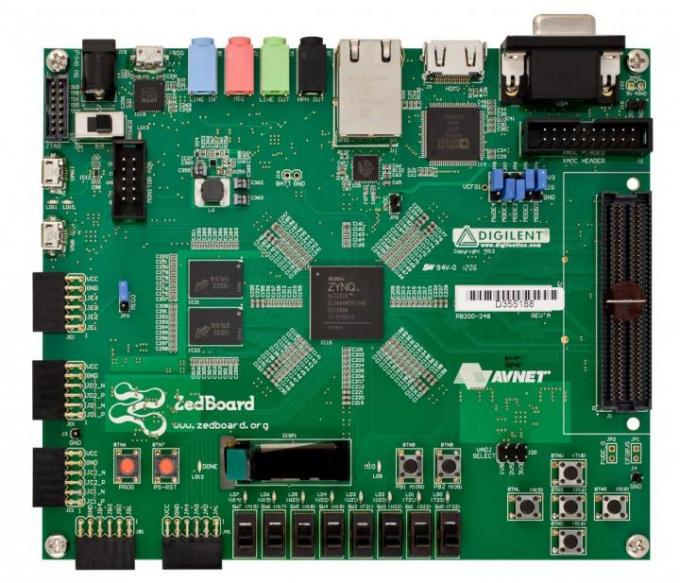
\includegraphics[width=8cm]{figuras/zedboard}
	\caption{Arquitetura do Zynq 7000.}
\end{figure}

\subsection{UART}
A UART (Universal Asynchronous Receiver/Transmitter) é um componente que trata da saída e entrada serial do sistema, portanto sendo o componente responsável por transmitir e receber caracteres, sendo necessário para impressão em tela, o que pode ser feito tanto por meio de um conector VGA quanto por USB (usado principalmente para depuração do código). As duas principais funções na classe da UART dentro do EPOS são justamente a put e get, para impressão e leitura de caractere, respectivamente. O Zynq possui duas UARTs.



\subsection{MMU} %http://epos.lisha.ufsc.br/EPOS+User+Guide#MMU

A MMU (\emph{Memory Managemed Unit}) é um componente responsável por gerenciar a memória de um sistema. É este componente o responsável por traduzir o endereçamento lógico em endereçamento físico. Uma das principais vantagens de seu uso é a possibilidade de proteção de memória.

%%%%%%%%
%		Get image from ug585 v1.7 p.79!
%%%%%%%%
\section{Ambiente de Desenvolvimento}

O ambiente de desenvolvimento usado para o porte foi o qemu para ARM (\verb+qemu-system-arm+), para executar o EPOS num ambiente virtualizado (emulado), pois assim pode-se usar ferramentas como o GDB para a depuração do código. O uso do GDB foi fundamental para o desenvolvimento, já que com ele era possível imprimir o valor de cada registrador em um dado ponto da execução, verificar a memória, executar instruções específicas e etc. Para compilar o EPOS foi usado \emph{cross-compilers} para ARM. As flags usadas para criar um ambiente de depuração com o qemu e o GDB foram as sequintes (com cada comando feito em um terminal diferente):
\begin{verbatim}
	qemu-system-arm -no-reboot -nographic -s -S -machine xilinx-zynq-a9\
	-cpu cortex-a9 -kernel ./img/zynq_app -fda ./img/zynq_app.img

	arm-none-eabi-gdb -ex "target remote :1234"
\end{verbatim}

O hardware real também estava disponível, e foi usado quando quando o qemu não produzia resultados confiáveis. Com o hardware real, para a depuração do código foi usado o JTAG.

\chapter{Porte}

% Eu poderia descrever como eu tenho que incluir cada classe feita em ./include/system/types.h, opções de traits, etc..


Nesta seção será discutido como foi o porte de cada mediador de hardware, explicando as decisões e dificuldades encontradas.

Antes de entrar nas especificidades de cada componente, é interessante colocar aqui alguns conceitos comuns que são usados em cada mediador.

A maneira usada para se comunicar, configurar e ler o estado de um dado componente de hardware é através da leitura e/ou escrita em registradores mapeados em memória. Um registrador mapeado em memória basicamente é uma região fixa da memória, onde uma escrita naquela posição indica uma escrita no registrador lá mapeado.
Exemplificando, a UART possui um registrador chamado rcvr\_timeout\_reg0, responsável por indicar quantos ciclos\footnote{Na realidade é o número de baud\_samples que se passaram.} a UART deve esperar um novo caractere chegar antes de emitir uma interrupção de \emph{timeout}. Este registrador está mapeado na posição de memória 0xE000001C para a UART0. Portanto, para configurar que o número de ciclos esperado seja de 20, basta escrever este número naquela posição. Uma maneira de fazer esta escrita, por exemplo, em C/C++, é: \verb+*((unsigned long*)0xE000001C) = 20;+.

%\section{memory map}

%\section{Boot}

\section{Traits}

Existem 4 arquivos traits.h que devem ser levados em consideração em um porte, dois deles devem ser completamente reescritos. Os arquivos \verb+./include/traits.h+ e \verb+/include/system/traits.h+ (onde '.' é a pasta raiz do código) possuem configurações gerais do EPOS, que, a princípio, devem ser independentes de arquitetura. Na prática há alguns pequenos ajustes que devem ser feitos nesses arquivos, pois é lá que se define, por exemplo, se o EPOS trabalhará em um processador \emph{multicore}, se utilizará \emph{scratchpad}, quais componentes estarão em modo de depuração e etc; entretanto isto se resume a trocar o valor de algumas variáveis de \emph{true} para \emph{false} ou o contrário.

Os outros dois arquivos são \verb+./include/mach/zynq/traits.h+ e \verb+./include/arch/armv7/traits.h+. Essa divisão é necessária pois, como dito anteriormente, é possível de um mesmo processador estar em diferentes \emph{machines}, e, caso seja necessário fazer um porte para esta plataforma, bastaria modificar os arquivos da pasta \emph{mach}, deixando os da pasta \emph{arch} praticamente intáctos, o que facilita muito novos portes.

Em \verb+./include/arch/armv7/traits.h+ trata das opções específicas do processador, portanto é lá que opções como \emph{endianess}, velocidade de \emph{clock}, número de \emph{cores}, tamanho da heap e stacks, bem como outras opções pertinentes ao mapeamento de memória e opções da MMU podem ser configuradas.

No arquivo de traits da \emph{machine}, ficam as opções de configuração de componentes como a UART, controlador de interrupções, \emph{timer}, e qualquer componente de interfaceamento externo à placa (rede, por exemplo). Componentes podem ser facilmente desativados nestas opções.

\section{Metaprogramação estática}

A arquitetura do EPOS usa pesadamente de metaprogramação estática para, em tempo de compilação, selecionar a arquitetura, bem como cada componente que será ou não utilizado. Por exemplo, podemos definir um \emph{if} estático para selecionar de qual classe a classe Chronometer irá derivar. Primeiramente a definição do \emph{if}:

\begin{verbatim}
template<bool condition, typename Then, typename Else> struct IF
{
    typedef Then Result;
};
\end{verbatim}

Este template, a princípio, nada mais faz do que tomar 3 parâmetros e então criar um tipo chamado Result igual ao segundo parâmetro, entretanto se nós fizemos uma especialização deste template, ele passa ser útil:

\begin{verbatim}
template<typename Then, typename Else> struct IF<false, Then, Else>
{
    typedef Else Result;
};
\end{verbatim}

Com esta especialização, toda vez que o primeiro parâmetro resolver-se como falso, Result será definido como o terceiro parâmetro. Temos, portanto, um \emph{if} metaprogramado funcional, agora voltemos ao exemplo do chronometro.

Suponha que caso a arquitetura não seja multicore, e nos traits o TSC (\emph{time stamp clock}) esteja ativo, então deseja-se que Chronometer derive de TSC\_Chronometer, do contrário de Alarm\_Chronometer.

Isto pode ser feito usando nosso \emph{if} metaprogramado da seguinte forma:

\begin{verbatim}
class Chronometer: public
IF<Traits<TSC>::enabled && !Traits<System>::multicore,
TSC_Chronometer, Alarm_Chronometer>::Result
{//class body};
\end{verbatim}

Deste modo, Chronomometer derivará de IF::Result, que será resolvido como TSC\_Chronometer ou Alarm\_Chronometer. Note que esse exemplo também mostra um uso do Traits, onde para descobrir se o TSC está ativo, bastou ler a constante Traits<TSC>::enabled, e para saber se o sistema é multicore bastou ler Traits<System>::multicore. Todo esse processamento causa zero \emph{overhead} em tempo de execução.

\section{Porte da UART}

A inicialização da UART foi feita de acordo com o sugerido pelo manual em \cite[p.~554]{ug585}. Nesta seção será comentado as decisões tomadas na configuração inicial da UART, em particular por causa dos momentos em que o manual exigia que o desenvolvedor tomasse uma decisão.

A primeira decisão que foi necessária é a de escabelecer qual será a taxa de transmissão (\emph{Baud Rate}) da UART. 

\begin{figure}[ht!]
    \centering
    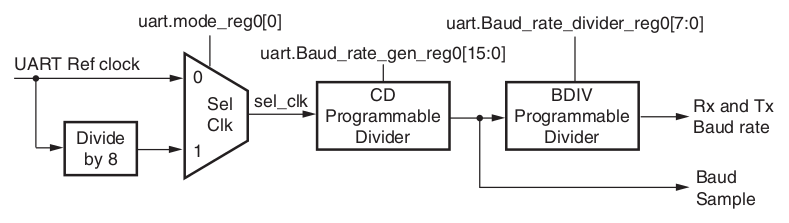
\includegraphics[width=10cm]{figuras/uart_board_rate}
    \caption{Esquemático de como é criada a taxa de transmissão.}
	\label{fig:uart}
\end{figure}

Primeiramente foi necessário configurar o \emph{clock} de referência da UART. Para isto, deve-se dividir o \emph{clock} que vem do I/O PLL (que por sua vez deriva do PS\_CLK, que é o \emph{clock} geral do sistema). Recomenda-se dividir o \emph{clock} da I/O PLL de modo a se obter 50 ou 33 MHz.
O \emph{clock} da I/O PLL, por padrão, multiplica o PS\_CLK (de 33.33 MHz) por 26, resultando num \emph{clock} de 866 MHz.
No manual diversas vezes é usado como exemplo para o \emph{clock} de referência da UART 50 MHz, portanto, arbitrariamente, escolheu-se esse valor. Logo, deve-se configurar o registrador UART\_CLK\_CTRL, responsável por configurar o \emph{clock} de entrada da UART, para dividir este \emph{clock} vindo da I/O PLL por 17 ($866/17 = 50$).

Agora, com este \emph{clock} estabelecido, que vamos chamar de sel\_clk (de acordo com a nomenclatura do manual), devemos calcular quanto será a taxa de transmissão.
Após alguma pesquisa em fóruns de desenvolvedores de software básico, notei que uma taxa de transmissão de 9600 bps é o mais comum, portanto, assumindo este valor, a próxima etapa é configurar os dois divisores de \emph{clock} que ajustam a taxa de transmissão, como indicado na figura \ref{fig:uart}.

O primeiro divisor chama-se CD (\emph{clock divider}), que configura a constante para se dividir o \emph{clock}, e BDIV um segundo divisor usado para sobreamostragem, organizado como mostrado na figura \ref{fig:uart}. O valor da taxa de transmissão final é calculado da seguinte forma:
\begin{equation}
	\text{taxa de transmissão} = \frac{sel\_clk}{CD \times (BDIV+1)}
\end{equation}

O valor padrão de BDIV é 15, portanto, fixiando-se esse valor e resolvendo a equação por CD, temos que $CD = 325$. Configurando-se estes valores nos seus respectivos registradores, obtém-se a taxa de transmissão desejada de 9600 bps.

Após estas configurações, dentre outras que o manual descreve, a UART está pronta para ser usada. Os dois principais métodos usados da UART são o put e o get, o primeiro escreve um caractere na saída serial, sendo que este pode ser lido, por exemplo através de uma entrada USB, para imprimir estes caracteres numa tela; algo muito útil para depuração.

\section{Porte do \emph{timer}}



Um \emph{timer} permite contar um certo número de ciclos, e, ao final da contagem, ele emite uma interrupção ao GIC, para que então o processador trate este evento. Entretanto note que é possível de existir mais \emph{timers} sendo usados logicamente do que \emph{timers} físicos disponíveis, significando que um mesmo \emph{timer} deve conseguir servir a mais de uma requisição simultaneamente.

Portanto não podemos apenas configurar um \emph{timer} para contar initerruptamente até passar o tempo que desejamos, do contrário novas requisições sobreescreveriam a anterior. Para ilustrar, suponha que se queira contar por 10 segundos, como o \emph{clock} do \emph{timer} é de 333 MHz (periodo $1/333 \times 10^6$), bastaria configurar o \emph{timer} para contar por $10 \times 333 \times 10^6$ ciclos e então chamar o \emph{handler} associado a interrupção gerada quando o \emph{timer} chegar em zero.

Agora imagine que, no cenário acima, enquanto o \emph{timer} ainda está servido àquela solicitação de contagem, apareça outra solicitação, de um alarme por exemplo, e queria contar por 20 segundos. Se esta solicitação sobrescrever o registrador de configuração do \emph{timer}, a solicitação anterior não terá seu pedido atendido a tempo. Note também que o escalonador de processos também estará usando este \emph{timer}.

Para resolver este problema, na arquitetura do EPOS existe o conceito de ticks (algo parecido com o que se faz no Linux), onde se configura um \emph{timer} para gerar interrupções em um intervalo regular, intervalo este que deve ser pequeno o suficiente para poder atender a demanda de contagens de pequenos valores, assim como não ser pequeno demais ao ponto de gastar mais processamento tratando as interrupções geradas pelo \emph{timer} do que servindo à outras funções. Assim, cada objeto que instancia (ou usa) um \emph{timer}, como o Alarm, Scheduler e Chronometer, nunca realmente tocam em algum registrador do \emph{timer} (portanto esses componentes são independentes de arquitetura), e, no lugar disso, computam quantos ticks, isto é, quantas interrupções de \emph{timer} aconteceram.

Para exemplificar o funcionamento destes componentes, tomemos o escalonador de processos. No construtor do escalonador, é enviado como parâmetro o periodo de escalonamento, ou seja, quanto tempo (no máximo) uma thread pode executar antes de ser escalonada. Para se saber quantos ticks devem ser contados antes de se escalonar um processo, basta dividir a frequência em que os ticks incrementam, pela frequência de escalonamento. Por exemplo, se o timer gera uma interrupção a cada 1 milisegundo (1000 Hz), e o escalonador escalona um processo a cada 10 milisegundos (100 Hz), o número de ticks a se contar é $1000/100 = 10$ ticks. Estes são os valores usados na implementação também.

No caso do Alarm em específico, internamente há uma fila com todas as requisições de alarme, ordenado do menor tick ao maior. Quando ocorre uma interrupção de timer, é chamado primeiramente o \emph{handler} que gerencia esta fila, e, caso um alarme desta fila já tenha esperado os ticks que requisitou, então o \emph{handler} desse alarme é chamado (este \emph{handler} é definido pelo usuário que instanciou o alarme).


O construtor do \verb+Zynq_Timer+ recebe como parâmetro a frequência que o contador deve contar, assim como o \emph{handler} que deve ser chamado quando esta contagem terminar (isto é, a função chamada quando acontecer uma interrupção devido ao timer ter chego a zero), e um número chamado channel, que serve para demultiplexar qual handler deve ser chamado.

A classe \verb+Zynq_Timer+ possui um atributo estático (e portanto único para todas as instâncias) definido como \verb+Zynq_Timer*+ \verb+_channels[CHANNELS]+, onde \verb+CHANNELS+ é uma constante com o número de diferentes classes usando o \emph{timer} (Scheduler e Alarm). Este vetor é necessário pois, quando uma interrupção de \emph{timer} acontece e o \emph{handler} do \emph{timer} é chamado, o \emph{handler} pode iterar sobre ele, chamando todos os respectivos \emph{handlers} daquelas classes.


Os 4 principais registradores a se trabalhar para configurar o \emph{timer} são o \verb+load+, registrador onde se escreve por quantos ciclos se deve contar; o \emph+counter+, que é o registrador que contém o atual valor contado, sendo decrementado a cada ciclo até chegar em zero, chegando em zero o é gerada uma interrupção número 29; registrador \emph+control+, que permite configurar certos comportamentos do \emph{timer}, como o de ativa-lo, ativar modo cíclico, ativar interrupções e atribuir um valor para o \emph{prescale}; e finalmente o registrador \emph+interrupt status+, que, como o nome indica, permite que se leia o status das interrupções de timer. Todos os timers trabalham à metade do \emph{clock} do sistema, ou seja, usando o \emph{clock} CPU\_3x2x.

Durante a inicialização do sistema, o \emph{timer} é configurado para gerar interrupções periodicamente, e esta configuração não é alterada durante a execução da aplicação. Como o construtor do \verb+Zynq_Timer+ recebe uma frequência como parâmetro, é necessário se converter esta frequência para um número de ciclos a se contar. Para isto, é necessário se levar em conta a frequência com que o contador é decrementado, para então se definir um valor a ser decrementado periodicamente de modo a fornecer a frequência desejada.

Como sabemos que o \emph{clock} ao qual o \emph{timer} está submetido é metade do \emph{clock} do sistema, e que antes dele chegar ao contador, este mesmo clock é dividido por um divisor chamado \emph{prescaler} (que divide pelo valor configurado nele mais 1), podemos dizer que:
\[
	COUNTER\_CLOCK\_FREQUENCY = \frac{SYSTEM\_CLOCK}{2 \times (PRESCALER+1)}
\]
Logo, usando a mesma linha de racioncínio exposta no exemplo de cálculo de ticks, temos que o valor a ser carregado no \verb+load_register+ (que será chamado de \verb+load_value+), sendo a frequência desejada F, é:
\begin{equation}
	\text{load\_value} = \frac{SYSTEM\_CLOCK}{2 \times (PRESCALER+1) \times F}
\end{equation}


Precisamos agora definir o prescaler. Definimos ele como a razão entre o \emph{clock} do \emph{timer} pela frequência desejada ($\frac{\text{clock}}{2 \times F}$). Há a premissa de que a frequência desejada não será maior que a do \emph{clock} do \emph{timer}, pois é impossível contar mais rápido que isto. Normalmente esta razão ($\frac{\text{clock}}{2 \times F}$) será um número maior que 255, já que o clock costuma ser muito mais rápido, e como o campo onde se registra o valor do prescaler possui apenas 8 bits, frequentemente o prescaler será 255.



\section{Mapeamento de Memória}

Por padrão, as 8 primeiras palavras da memória (ou seja, $8 \times 4 = 32$ bytes) devem possuir instruções específicas. A primeira palavra (memória posição 0) contém a primeira instrução a ser executada, e, nas 7 palavras seguintes, fica a tabela de vetores (\emph{vector table}). Como abaixo da instrução inicial há uma tabela que não se deseja executar no momento de inicialização do sistema, esta primeira instrução necessariamente é um \emph{jump} para uma outra região, para aí então se iniciar o processo de \emph{boot}. 
As demais 7 palavras, pertencentes à tabela de vetores possuem, similarmente, \emph{jumps} para o código onde o tratador da exceção se localiza. A primeira instrução da tabela (posição 0x4) deve conter um \emph{jump} o tratador de uma exceção do tipo undefined instruction, depois, na próxima palavra, a software interruption, prefectch abort, data abort, reserved, irq e, finalmente, fiq, nesta ordem. Vide seções \ref{sec:interrupt} e \ref{sec:operating_modes} para mais detalhes.


%desmontamento do binário da imagem do EPOS
Desmontando-se o binário da imagem produzida na compilação do EPOS (\emph{dump}), deve-se obter uma saída semelhante a esta exemplificada abaixo em seus primeiros 32 bytes:

\label{dump}
\hspace*{-1.8cm}\vbox{
\begin{verbatim}
	00000000 <_vector_table>:
		 0:	e59ff7fc 	ldr	pc, [pc, #2044]	; 804 <_start_addr>
		 4:	e59ff7fc 	ldr	pc, [pc, #2044]	; 808 <_undefined_instruction_addr>
		 8:	e59ff7fc 	ldr	pc, [pc, #2044]	; 80c <_software_interrupt_addr>
		 c:	e59ff7fc 	ldr	pc, [pc, #2044]	; 810 <_prefetch_abort_addr>
		10:	e59ff7fc 	ldr	pc, [pc, #2044]	; 814 <_data_abort_addr>
		14:	e59ff7fc 	ldr	pc, [pc, #2044]	; 818 <_reserved_addr>
		18:	e59ff7fc 	ldr	pc, [pc, #2044]	; 81c <_irq_handler_addr>
		1c:	e59ff7fc 	ldr	pc, [pc, #2044]	; 820 <_fiq_handler_addr>
\end{verbatim}
}

Também foi necessário definir as pilhas (\emph{stacks}) do sistema, assim como reservar um espaço para a pilha dos tratadores de interrupção. O \emph{layout} escolhido segue na tabela \ref{tab:stacks}.
Este é o \emph{layout} usado durante o desenvolvimento. Somente as pilhas de usuário e de algum modo privilegiado (como o supervisor) são necessárias, portanto a pilha de supervisor acabaria por englobar as demais posições que aparecem na tabela \ref{tab:stacks}. Na próxima seção é explicado como foi feito para não precisar reservar espaço na memória para as demais pilhas.

\begin{table}[hb]
	\centering
	\begin{tabular}{ccc}
		\hline \hline
		Pilha & Endereço base & Tamanho máximo (bytes)\\[0.5ex]
		\hline
		Supervisor		& \verb+0x00100000+ & 983040\\
		Irq			& \verb+0x00100040+ & 64\\
		System			& \verb+0x00100080+ & 64\\
		Abort			& \verb+0x001000c0+ & 64\\
		Fiq			& \verb+0x00100100+ & 64\\
		Undefined		& \verb+0x00100140+ & 64\\[1ex]
		\hline
	\end{tabular}
	\caption{Pilhas do sistema com seus tamanhos e posições.}
	\label{tab:stacks}
\end{table}

Lembrando que pilhas, num sistema operacional, tradicionalmente crescem em direção à posições menores da memória, por isto que, por exemplo, a pilha Irq possui 64 bytes, já que $\texttt{0x100040}-\texttt{0x100000} = 40_{16} = 64_{10}$. A pilha do usuário, portanto, localiza-se na última posição da memória (512 MB neste caso) e cresce para ``baixo'' (posições menores de memória) a partir de lá.

%Falar da heap.
%Memory top/base, app_code, app_data...


%%>>>>>continue from here
Restante do mapeamento de memória:
\ref{tab:mem}.
\begin{table}[hb]
	\centering
	\begin{tabular}{ccc}
		\hline \hline
		Dado & Endereço base & Tamanho máximo\\[0.5ex]
		\hline
		Tabela da MMU		& \verb+0x00100144+ & ~5mb\\
		APP\_DATA		& \verb+0x00600000+ & 1mb\\
		SYS\_HEAP		& \verb+0x00700000+ & 32mb\\
		APP\_HEAP		& \verb+0x02700000+ & \\
		APP\_STACK		& \verb+0x1ffffffc+ & \\[1ex]
		\hline
	\end{tabular}
	\caption{Pilhas do sistema com seus tamanhos e posições.}
	\label{tab:stacks}
\end{table}


\section{Porte do Controlador de Interrupções}

%falar sobre os handlers, qual a sequência de chamadas de função
%int_vector
%os diferentes tipos de interrupção (abort, prefetch...), dar exemplos de quando são gerados
%ICCIAR and ICCEOI register
%spurious interruption 1023
%explicar approach usado em exception.cc

Para se usar o controlador de interrupções (que será referenciado como GIC no restante desta seção, de \emph{Generic Interrupt Controller}), é necessário antes inicializar o distribuidor de interrupções e as interfaces dos processadores.

É no distribuidor que é determinada a prioridade de cada interrupção, e onde é decidido se determinada interrupção deve ou não ser encaminhada para a interface de um determinado processador. Todas as interrupções passam por ele.

A interface dos processadores é por onde os processadores se comunicam com o GIC. Nela o processador confirmar que recebeu a interrupção (\emph{acknowledge}), indicar que terminou de tratar a mesma, definir prioridades entre diferentes interrupções, indicar uma política de preempção de interrupções, ou mesmo desligar esta interface. Como o GIC é dividido logicamente é ilutrado na imagem \ref{img:gic}

\begin{figure}[ht!]
    \centering
    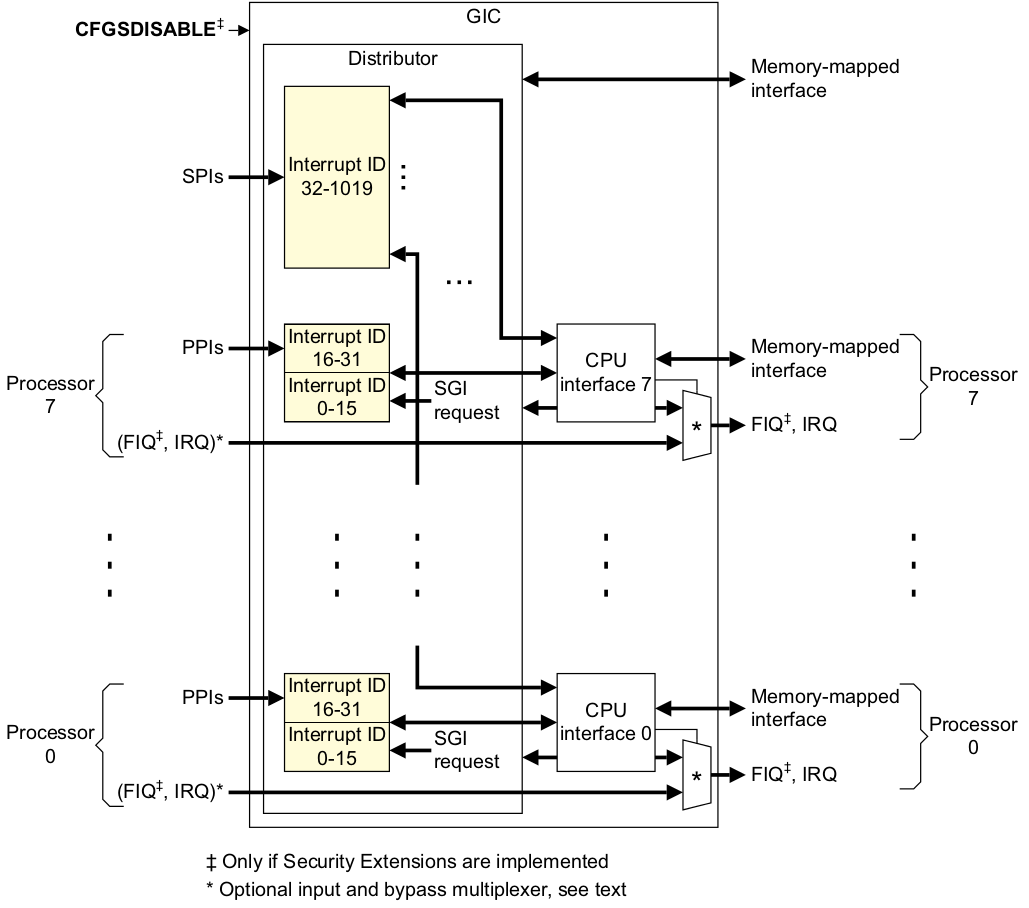
\includegraphics[width=8cm]{figuras/gic}
    \caption{Divisão lógica do GIC.}
    \label{img:gic}
\end{figure}

\subsection{Inicialização}

Na inicialização do distribuidor, através dos registradores mapeados em memória de configuração do mesmo, é definido, para cada uma das possíveis interrupções, se elas são \emph{level-sensitive} ou \emph{edge-triggered}.
Em seguida configura-se a prioridade de cada interrupção. A princípio todas as interrupções foram definidas como tendo a mesma prioridade, mas isto é configurável caso necessário.
É configurado então o processador-alvo de cada interrupção, isto é, para quais interfaces de processador uma determinada interrupção será encaminhada. Finalmente então são ativadas as interrupções.

A inicialização da interface do processador é mais simples. Primeiro se configura a máscara de prioridade da CPU, isto é, qual é o nível de prioridade mínimo que uma interrupção precisa ter para interromper aquele processador. Na implementação esta máscara está desativada. Depois configura-se a política grupos de preempção. No GIC é possível separar interrupções em grupos de preempção, onde se define se determinado grupo pode preemptar determinado outro grupo. Todas as interrupções foram colocadas no mesmo grupo e interrupções podem ser preemptadas.

Adicionalmente a estas configurações, é possível de mascaras as interrupções FIQ e IRQ através do CPSR (\emph{Current Program Status Register}), alterando-se os bits 6 e 7 dele, para mascarar interrupções FIQ e IRQ, respectivamente. Normalmente é o que é feito quando é necessário mascaras as interrupções, enquanto se mantém as configurações do GIC.

\subsection{Fluxo de execução ao se receber uma interrupção}

O processador, ao se receber uma interrupção, (e, portanto as interrupções estão ativas e não mascaradas pela interface ou pelo CPSR), o processador para a execução do código que estava executando e então executa a instrução contida na tabela de vetores (mostrada na página \pageref) correspondente ao tipo de interrupção recebida. Esta instrução é um jump para um tratador (\emph{handler}) daquele tipo de interrupção.

O principal tratador é o tratador de interrupções IRQ (\verb+irc_handler+), sendo que este precisa ser discutido com mais profundidade. Abaixo segue o código deste tratador:

\begin{verbatim}
 43 void _irq_handler() {
 44   ASMV(
 45   // A few definitions
 46   ".equ ARM_MODE_FIQ,      0x11 \n"
 47   ".equ ARM_MODE_IRQ,      0x12 \n"
 48   ".equ ARM_MODE_SVC,      0x13 \n"
 49   ".equ IRQ_BIT,           0x80 \n"
 50   ".equ FIQ_BIT,           0x40 \n"
 51 
 52   "msr cpsr_c, #ARM_MODE_SVC | IRQ_BIT | FIQ_BIT \n" // go to SVC
 53   // save current context (lr, sp and spsr are banked registers)
 54   "stmfd sp!, {r0-r3,r12,lr,pc}\n"
 55 
 56   "msr cpsr_c, #ARM_MODE_IRQ | IRQ_BIT | FIQ_BIT\n" //go to IRQ
 57 
 58   "sub r0, lr, #4 \n" // return from irq addr
 59   "mrs r1, spsr   \n" // pass irq_spsr to svc r1
 60 
 61   "msr cpsr_c, #ARM_MODE_SVC | IRQ_BIT | FIQ_BIT\n"//go back to SVC
 62   "add r2, sp, #24 \n"  // sp+24 is the position of the saved pc
 63   
 64   // save return address into the pc position
 65   "str r0, [r2] \n" 
 66   "stmfd sp!, {r1} \n"   // save irq-spsr
 67       
 68   );    
 69   
 70     
 71   IC::int_handler();
 72     
 73   ASMV(        
 74   "ldmfd sp!, {r0}              \n"
 75   "msr spsr_cfxs, r0 \n" // restore IRQ's spsr value to SVC's spsr
 76             
 77   "ldmfd sp!, {r0-r3,r12,lr,pc}^ \n" // restore context
 78   //the ^ in the end of the above instruction makes the 
 79   //spsr to be restored into svc_cpsr
 80   );
 81 }
\end{verbatim}

Após selecionar qual handler chamar, o processador muda de modo, indo, no caso de uma interrupção IRQ, para o modo de execução IRQ. Neste modo há 3 registradores banqueados: O SPSR, que contém o valor do registrador CPSR imediatamente antes da interrupção, sendo necessário para que seja possível restaurar o valor original do CPSR após tratar a interupção; o LR (link register), que contém o endereço da próxima instrução que seria executada imediatamente antes da interrupção mais 4; e, finalmente, o SP (stack register), que aponta para a pilha própria desde modo (cada modo pode possuir sua própria pilha).

Para evitar desperdício de memória reservando uma pilha própria apenas para este modo, optou-se por não usar uma pilha no modo IRQ, e, no lugar disto, usar sempre a mesma pilha do modo supervisor (que é o modo de exceução do processador quando ele inicia). Para isto, a primeira instrução a se executar é uma mudança de modo para voltar ao modo supervisor, enquanto mantendo novas interrupções desligadas; lá é salvo o contexto na pilha daquele modo. Entretanto para que seja possível restaurar o fluxo de execução no mesmo estado em que o processador estava no momento imediatamente antes da interrupção, é necessário voltar ao modo IRQ para obter-se os valores contidos dos registradores banqueados SPSR e LR; após isto, pode-se então voltar ao modo \emph{supervisor}. Na linha 62 do código é somado 24 à pilha pois lá é a posição de memória onde está salvo o PC após ele ter sido empilhado na linha 54, e deseja-se sobreescrever aquele valor do PC pelo valor que estava contido no LR do modod IRQ (menos 4), pois aquela é a próxima instrução que seria executada antes da interrupção. Feito isto, salva-se o valor do SPSR do modo IRQ no topo da pilha, para ser restaurado ao CPSR mais tarde. Agora que o contexto foi salvo corretamente para ser restaurado, pode-se então chamar um tratador de interrupções genérico (que será discutido mais a frente) e escrito em C++. Após o o \verb+int_handler+ da linha 71 retornar, é feita a restauração do contexto. Primeiro se salva o CPSR no SPSR, na última instrução (ldmfd), na forma em que ela está (com um ^ no final dela e com o PC na lista), ela automaticamente restaurará o valor que está no SPSR para o CPSR. Como o PC está na lista, o fluxo de execução terá retornado a executar as instruções de antes da interrupção ocorrer.

Agora será discutido como que as interrupções são tratadas individualmente. O corpo do \verb+int_handler+ é bastante curto, então vale a pena escreve-lo aqui.

\begin{verbatim}
void Zynq_IC::int_handler()
{	
    unsigned int icciar_value = CPU::in32(IC::GIC_PROC_INTERFACE 
    	| IC::ICCIAR);
	IC::Interrupt_Id id = icciar_value & IC::INTERRUPT_MASK;

	if(id == 1023){
		kout << "Spurious interruption received\n";
		return;
	}
    _vector[id](id);
    CPU::out32(IC::GIC_PROC_INTERFACE | IC::ICCEOI, icciar_value);
}
\end{verbatim}

A primeira coisa que o tratador faz e descobrir qual é o número da interrupção que foi gerada, para assim saber como tratar aquela interrupção. Isto é feito lendo-se o registrador ICCIAR (\emph{Interrupt Acknowledge Register}), que provê o número da interrupção e também o processador endereçado.
É possível que uma interrupção já tenha sido tratada por outro processador, quando isto acontece, o GIC emite uma \emph{Spurious Interruption} para indicar isto. Quando se detecta isto, o tratador não precisa tomar nenhuma outra ação, basta retornar a execução normal.

Com o número da interrupção em mãos, pode-se então chamar o tratador daquele tipo de interrupção. \verb+_vector+ é um vetor de \emph{handlers}, onde para cada posição $i$, existe o tratador da interrupção número $i$. Para sinalizar que uma interrupção foi tratada, deve escrever no registrador ICCEOI (End of Interruption) o número lido no ICCIAR (ou seja, o número da interrupção e processador de destino).


Normalmente, interrupções de \emph{timer} é o tipo mais frequente de interrupção durante a execução do sistema. Dele dependem o escalonador de processos (ou \emph{threads}), Delay, Chronometer e Alarm. Como mencionado na seção do porte do \emph{timer}, uma mesma interrupção pode gerar a chamada de mais de um handler, como a do \emph{timer} que chama a do Alarm e do escalonador.

\subsection{}


\bibliographystyle{ufscThesis/ufsc-alf}
\bibliography{references}

%--------------------------------------------------------
% Elementos pós-textuais
%\apendice
%\chapter{Exemplificando um Apêndice}
%Texto do Apêndice aqui. 

%\anexo
%\chapter{Exemplificando um Anexo}
%Texto do anexo aqui.
\end{document}
